% ----------------------------------------------------------------------------------------\
% ---------------------------------------------------------------------------------------\
% --------------------------------------------------------------------------------------\
\section{Investigación}
% ----------------------------------------------------------------------------------------\
% ---------------------------------------------------------------------------------------\
% --------------------------------------------------------------------------------------\

\subsubsection*{¿Qué es el algoritmo Genético?}

Un algoritmo genético \texttt{(AG)} entonces es: una técnica de resolución de problemas 
que utiliza principios inspirados en la selección natural para solucionar problemas de 
optimización. La selección natural (evolución) como estrategia implica la creación, 
reproducción y adaptación de una población de posibles soluciones en un rango de generaciones.\\ 

Este enfoque de población se basa en que cada individuo representa una posible solución 
al problema, y la evolución de estos comienza por, la \textbf{creación} de los individuos, 
la \textbf{reproducción} para después hacer la óptima \textbf{selección} de los padres en 
una nueva reproducción y \textbf{mutación}, finalmente comprobar o evaluar su \textbf{aptitud}\\ 


\subsubsection*{Pasos que sigue}

\begin{center}
    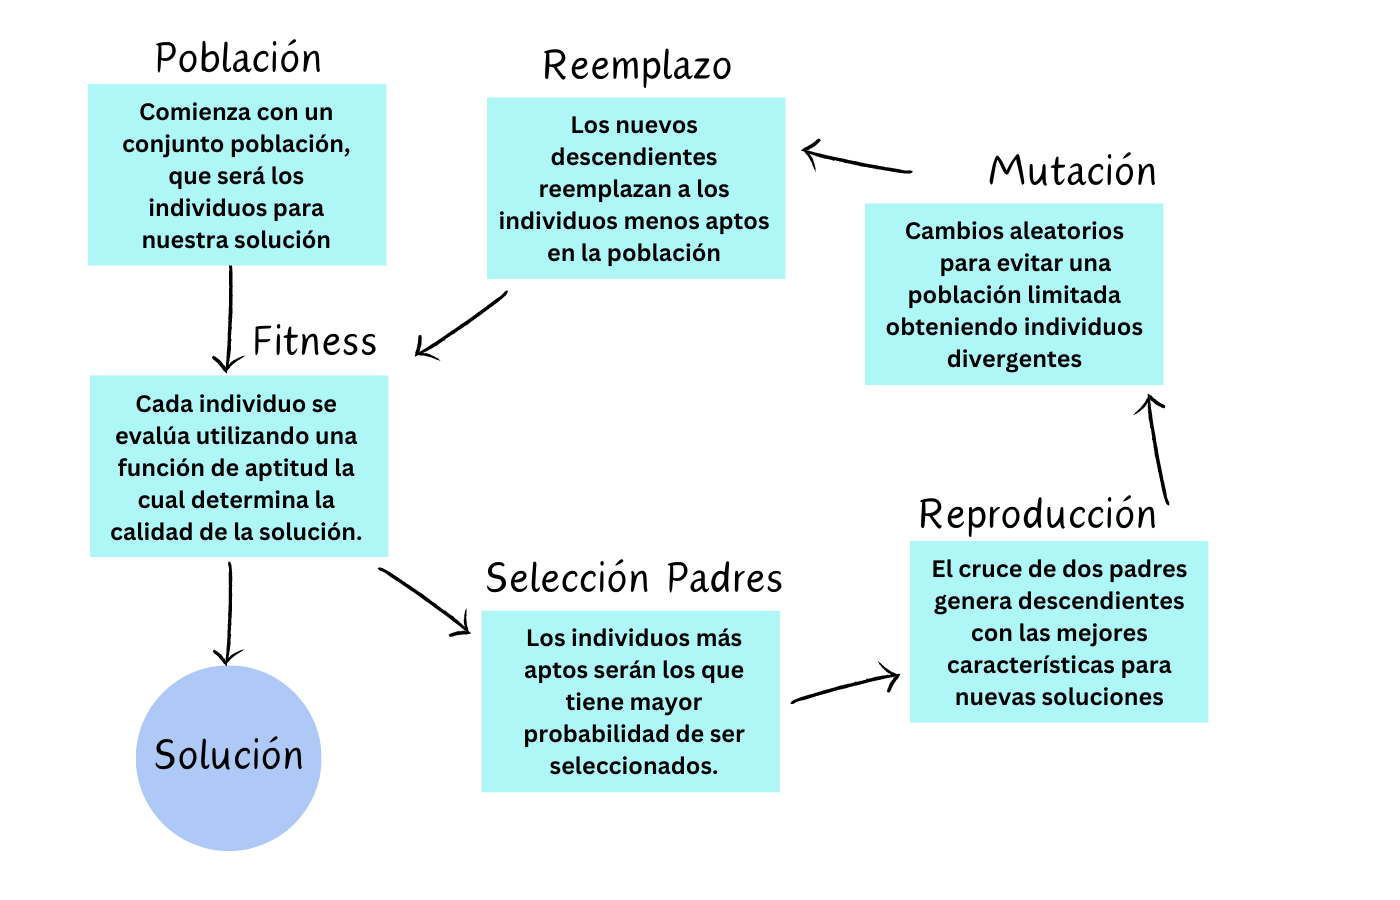
\includegraphics[scale = .35]{IMA/algo genetico.png}
\end{center}

\subsubsection*{¿Cuál es el juego de la vida?}

El Juego de la vida es un autómata celular, es decir es un modelo matemático llevado de 
manera computacional para observar de manera dinámica cómo evoluciona en el tiempo. Creado
por John Horton Conway en 1969 que consiste en una cuadrícula donde se marcan o desmarcan 
siendo pintados por un color, representando células y reflejando si esta se encuentra 
viva o muerta.\\ 


Iniciado el juego son las reglas las que determinan como acaba. El objetivo es crear un 
sistema que simulase la vida y su naturaleza. La manera en que se logra es con el nacimiento 
y supervivencia de estos seres binarios digitales donde depende del número de vecinos que 
estén a su vez vivos o muertos. Por lo que es posible observar patrones complejos e 
impredecibles gracias a unas sencillas reglas. Siendo utilizado como un modelo de simulación 
para estudiar fenómenos biológicos, evolutivos o físicos.

\begin{figure}[H]
    \centering
    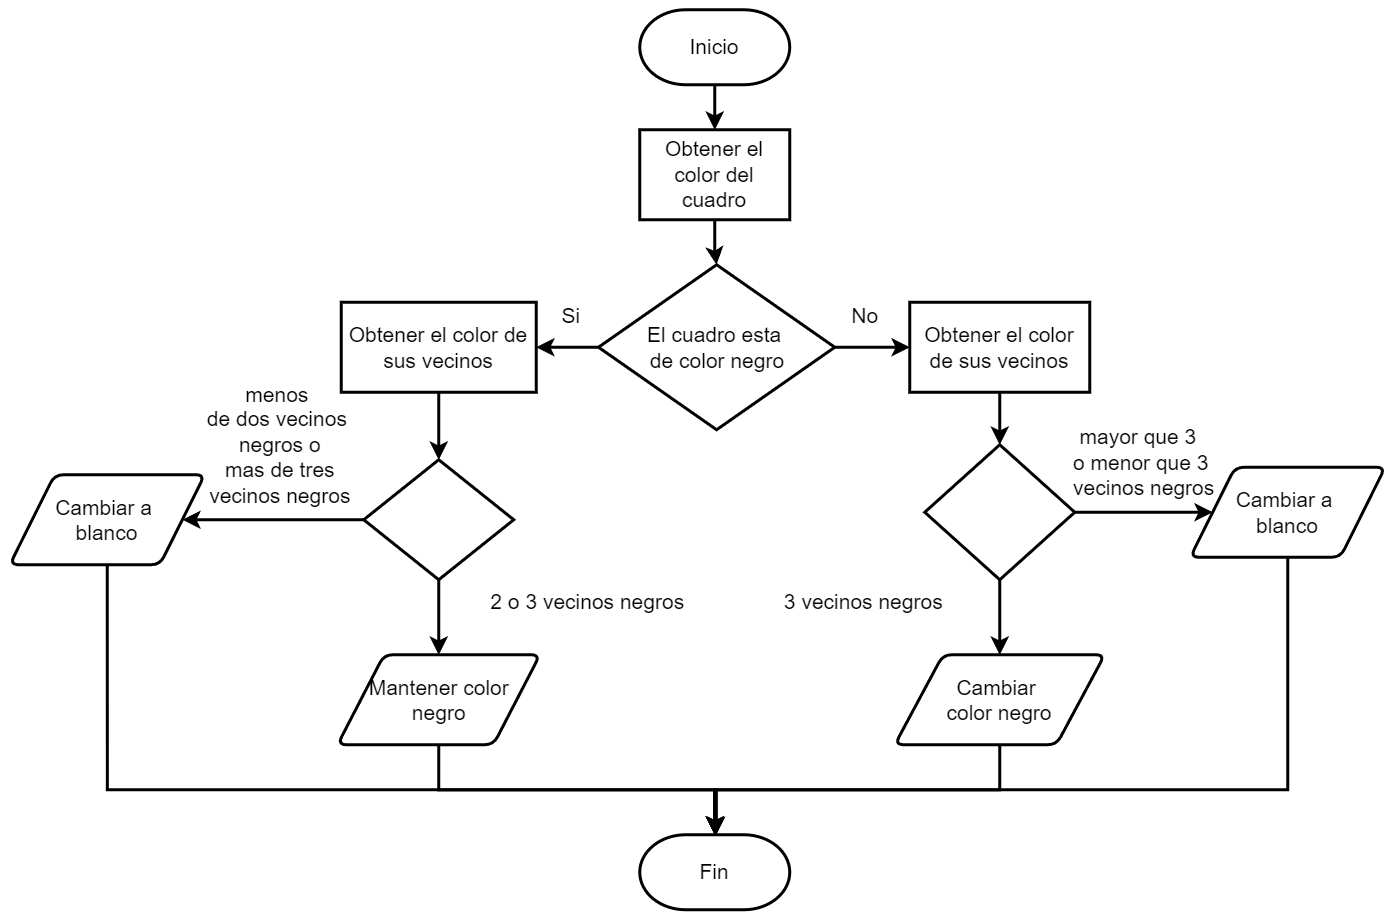
\includegraphics[width=0.9\linewidth]{IMA/DiagramaFlujoJuegoLaVida.png} 
    \caption{Diagrama de flujo del Juego de la Vida} 
\end{figure}

En el diagrama se puede observar las reglas que se siguen para determinar si una célula 
vive o muere. En este caso las condicionales del diagrama reflejan la sobrepoblación, la 
soledad , la reproducción y la supervivencia de las células. Por lo que solo faltaría 
implementar el código en Python para poder visualizar el juego de la vida.